\title{Final Exam for Algebra-Based Physics: Mechanics (PHYS135A)}
\author{Dr. Jordan Hanson - Whittier College Dept. of Physics and Astronomy}
\documentclass[10pt]{article}
\usepackage[a4paper, total={18cm, 27cm}]{geometry}
\usepackage{outlines}
\usepackage[sfdefault]{FiraSans}
\usepackage{graphicx}

\begin{document}
\maketitle
\small
\section{Equations and Constants}
Pythagorean theorem (magnitude of a vector): $|v| = \sqrt{v_x^2+v_y^2}$ \\
Dot-product of two vectors: $\vec{u} \cdot \vec{v} = uv\cos\theta = u_x v_x + u_y v_y$ \\
Displacement: $\Delta \vec{x} = \vec{x}_f - \vec{x}_i$ \\
Average velocity: $\vec{v} = \Delta \vec{x}/\Delta t$ \\
Average acceleration: $\vec{a} = \Delta \vec{v}/\Delta t$ \\
Kinematic equation 1 (constant acceleration): $v(t) = v_i + at$ \\
Kinematic equation 2 (constant acceleration): $x(t) = \frac{1}{2}at^2+v_i t+x_i$ \\
Kinematic equation 3 (constant acceleration): $v_f^2 = v_i^2 + 2 a \Delta x$ \\
Newton's First Law: if $\vec{F}_{Net} = 0$, $\vec{v} = const$ (or zero) \\
Newton's Second Law: $\vec{F}_{Net} = m \vec{a}$ \\
Newton's Third Law: $\vec{F}_{AB} = - \vec{F}_{BA}$ \\
Weight force: $\vec{w} = -mg\hat{j}$ \\
Normal force: $\vec{N} = +mg\hat{j}$ (unless surface is not flat) \\
Force of friction: $\vec{f}_f = -\mu \vec{N}$ \\
Drag force: $F_D = \frac{1}{2}C\rho A v^2$ \\
Terminal velocity: $v_T = \sqrt{(2mg)/(C\rho A)}$ \\
Definition of the radian: $s = r \theta$ \\
Angular velocity (change in radians per unit time): $\omega = \Delta \theta/\Delta t$ \\
Angular velocity (change in $\omega$ per unit time): $\alpha = \Delta \omega/\Delta t$ \\
Tangential velocity: $v = r\omega$ \\
Tangential acceleration $a = r\alpha$ \\
Centripetal acceleration: $a_c = r\omega^2 = v^2/r$ \\
Centripetal force: $F_c = m a_c$ \\
Newton's Law of Gravity: $F_G = G m_1 m_2 / r^2$, $G = 6.674\times 10^{-11}$ N m$^2$ kg$^{-2}$ \\
Kepler's 3rd Law (explicit): $r^3/T^2 = \frac{G}{4\pi^2} M$, where $M$ is the mass of the central body. \\
Kepler's 3rd Law (scaling): $r_1^3/T_1^2 = r_2^3/T_2^2 = const$ \\
Definition of Work: $W = \vec{F} \cdot \vec{d} = Fd\cos\theta$ \\
Definition of kinetic energy: $KE = \frac{1}{2} mv^2$ \\
Work-Energy theorem: $W = \Delta KE$ \\
Definition of gravitation potential energy: $U = mgh$ \\
Conservation of energy: $KE_i + U_i = KE_f + U_f$ \\
Power: $P = W/T = E/T$ \\
Conservation of momentum: $\vec{p}_{i,1} + \vec{p}_{i,2} = \vec{p}_{f,1} + \vec{p}_{f,2}$ \\
\clearpage
\section{Kinematics}
\begin{enumerate}
\item We are tracking a drone through Whittier College.  The drone begins on top of the Science and Learning Center (SLC).  It proceeds North towards Platner Hall, traveling 150 m in 10 seconds.  Next, it heads South for 120 m for 12 seconds.  (a) What are the velocities of the two segments of the flight? (b) What is the total distance traveled? (c) What is the displacement? \textit{(Hint: it's not the same as the total distance)}. (d) What is the average velocity over the whole flight? \\ \vspace{2.5cm}
\item Suppose a basketball player is shooting the ball.  The ball is 4.5 m from the hoop, horizontally.  The ball starts at the player's shoulder, 2.0 m above the ground.  The hoop is 3.0 m above the ground.  The shot goes in 1.25 seconds after the player shoots.  (a) Draw a diagram of the ball's trajectory. (b) What is the horizontal speed of the ball? (c) What is the vertical displacement of the ball at the moment it goes in the hoop? (d) What is the initial vertical speed of the ball? \\ \vspace{2.5cm}
\end{enumerate}
\section{Newton's Laws and Various Forces}
\begin{enumerate}
\item (a) What is the magnitude of $\vec{F}_{app}$ in Fig. \ref{fig:mouth} if the tension in the wire $T$ is 25.0 N?  (b) Suppose the gum applies to the tooth a force of 12 N in the opposite direction of $\vec{F}_{app}$.  What is the net force on the tooth?
\begin{figure}[hb]
\centering
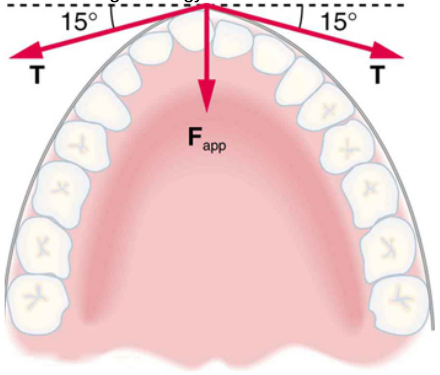
\includegraphics[width=0.25\textwidth]{figures/mouth.png}
\caption{\label{fig:mouth} Braces apply a net force on a tooth.}
\end{figure} \\
\item An object is sliding down an inclined surface with friction coefficient $\mu_k$. (a) Draw the free-body diagram.  (b) Show that the acceleration is given by $a = g(\sin\theta-\mu_k \cos\theta)$.  (c) If $\theta=25^{\circ}$ and $a=0.1$ m/s$^2$, what is $\mu_k$? \\ \vspace{2.5cm}
\item A meteorite is flying through space at constant velocity, but then accelerates because it is pulled towards the Earth by gravity.  When it enters the atmosphere it reaches \textit{terminal velocity} before it burns up. (a) Sketch a curve that describes the velocity versus time of the meteorite.  (b) Assume the drag coefficient and area of the object are $C=0.5$ and $A=4$ m$^2$, and that $\rho_{air} = 1.225$ kg/m$^3$.  What is the terminal velocity of the object if it has a mass of 5000 kg? \\ \vspace{3cm}
\end{enumerate}
\section{Rotational Motion and The Law of Gravity}
\begin{enumerate}
\item Assume that Earth has an orbital period of 1.0 year, and an orbital radius of 1.0 AU.  The orbital period of Saturn is observed to be about 29 years.  How far from the Sun is Saturn (in AU)? (b) The orbital radius of Mars is about 1.5 AU.  What is the duration of the orbit of Mars, in years? \\ \vspace{1.5 cm}
\item A polisher in a machine shop is a rough wheel that spins, grinding surfaces until they are smooth.  (a) If the wheel turns at 360 rpm, and has a radius of 5 cm, what is the tangential velocity at the surface of the wheel? (\textit{Be careful with units}). (b) If the angular velocity of the wheel is accelerated from 360 to 720 rpm in 1.0 second, what is the angular acceleration? \\ \vspace{1.0cm}
\end{enumerate}
\section{Work and Momentum}
\begin{enumerate}
\item Consider Fig. \ref{fig:work}.  (a) Is work being done in either situation?  Explain why or why not in your own words. (b) Suppose the man lifts the briefcase against gravity, through a distance of 1.0 m.  If the briefcase weighs 1.5 kg, how much work has the man done? (c) If he drops the briefcase from a height of 2.0 m, what will be the final kinetic energy and velocity?
\begin{figure}[hb]
\centering
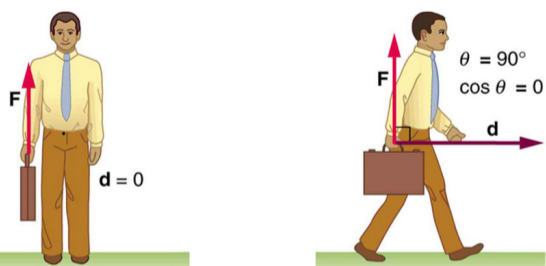
\includegraphics[width=0.5\textwidth]{figures/final1.png}
\caption{\label{fig:work} Two different scenarios regarding physical work.}
\end{figure}
\item The swimmer shown in Fig. \ref{fig:work} exerts an average horizontal force of 80.0 N during each 1.80 m long stroke. (a) What is his work output in each stroke? (b) Calculate the power output if each stroke takes 0.5 seconds.
\begin{figure}[hb]
\centering
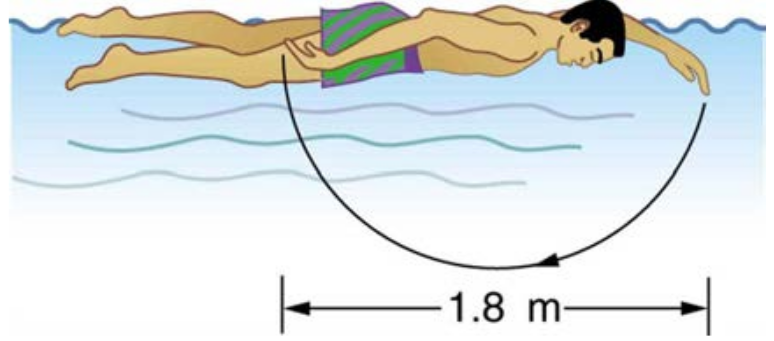
\includegraphics[width=0.5\textwidth]{figures/swim.png}
\caption{\label{fig:power} A swimmer exerts a force through a distance, doing work on the water.}
\end{figure}
\item Suppose an asteroid ejects a small chunk of mass.  Let the small chunk after the separation have a mass $m_1$, and the new mass of the asteroid be $m_2$.  Assume that initial velocity of the asteroid is zero.  Let the final velocities of the small chunk and asteroid be $v_1'$ and $v_2'$, respectively. (a) Show that the speed of the main asteroid after the separation is $v_2' = \left(\frac{m_1}{m_2}\right) v_1'$. (b) If we observe $v_1' = 100$ m/s, and $v_2' = 1$ m/s, and estimate that $m_1 = 1000$ kg, what is $m_2$?
\end{enumerate}
\end{document}